\chapter{Results}

\section{Intensity of Single Source - Diffraction}

Using python, I plotted distance vs. intensity for a single source. The relevant python code can be found in appendix \ref{code:single}.

\begin{figure}[!h]
\centering	
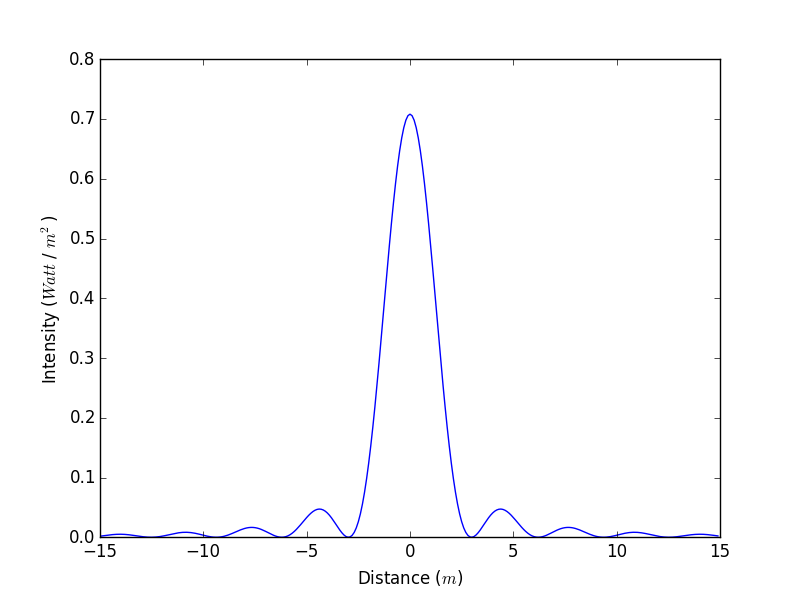
\includegraphics[scale=0.45]{figure_1.png}
\caption{Intensity profile of single antenna}
\end{figure}

\subsection{Discussion}

Here we have a single isotropic antenna source, radiating over a sphere centered on the source. It's intensity decreases as the lateral distance increases as it should (according to the inverse square law), because we have a spherical wave moving radially. In the center of the screen we have maximum intensity because that is the closest point to the source. 


\section{Intensity of Linear Array of 4 Antennae}

Plot between distance and intensity, for four antenna sources arrange in a linear array, all of them being in phase. It is immediately obvious that we have an interference pattern. The relevant code can be found in appendix \ref{code:four}.

\begin{figure}[!h]
	\centering	
    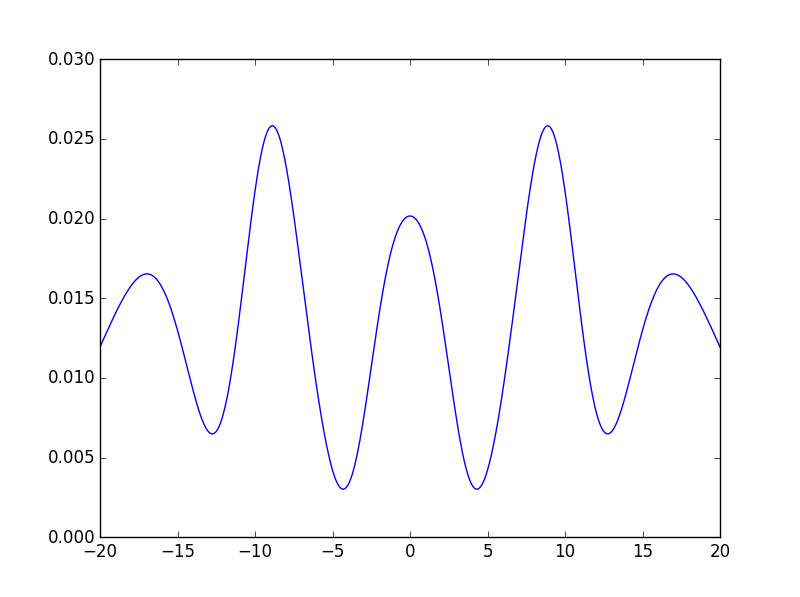
\includegraphics[scale=0.45]{figure_2.png}
	\caption{Intensity profile of linear array of 4 antennae}
\end{figure}

\subsection{Discussion}
We have 4 antenna sources arranged in a linear array. We get this radiation pattern by the contribution of all the antenna sources in the array. We get different lobes because of interference. Wherever spherical waves coming from each individual antenna source arrive in phase they add together (constructive interference) to enhance the intensity and where they arrive out of phase, with the peak of one coinciding with the another, the waves cancel (destructive interference) reducing the intensity in that direction.

\subsection{Managing Phase}

We used the same linear array of 4 antenna sources but modified the phase between them. Fig. (\ref{fig:phase_1}) (created using code \ref{code:phase_right}) corresponds to three antennas in phase and the right-most antenna completely out of phase ($\pi$ radians). Note how the intensity profile is no longer symmetric but in fact is shifting to the right. 

Fig. (\ref{fig:phase_2}) (created using code \ref{code:phase_left}) corresponds to the left-most antenna being completely out of phase while the remaining three are exactly in phase. The peak intensity shifts to the left. It is clear that by changing the phase we are steering the direction of peak intensity, that is, steering the beam.

\begin{figure}[!h]
	\centering	
	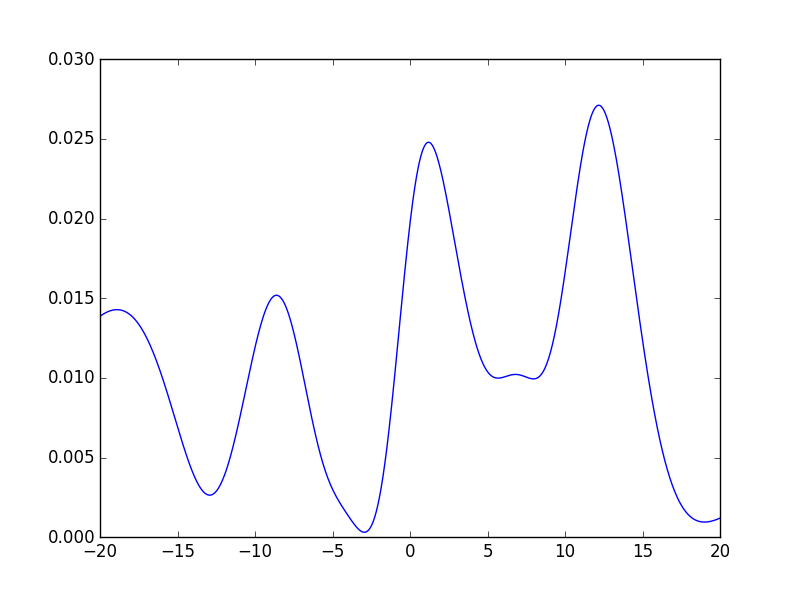
\includegraphics[scale=0.45]{figure_3.png}
    \caption{\label{fig:phase_1} Intensity profile of linear array of 4 antennae with 3 antennae in-phase and right-most antenna completely out of phase.}
\end{figure}

\begin{figure}[!h]
	\centering	
	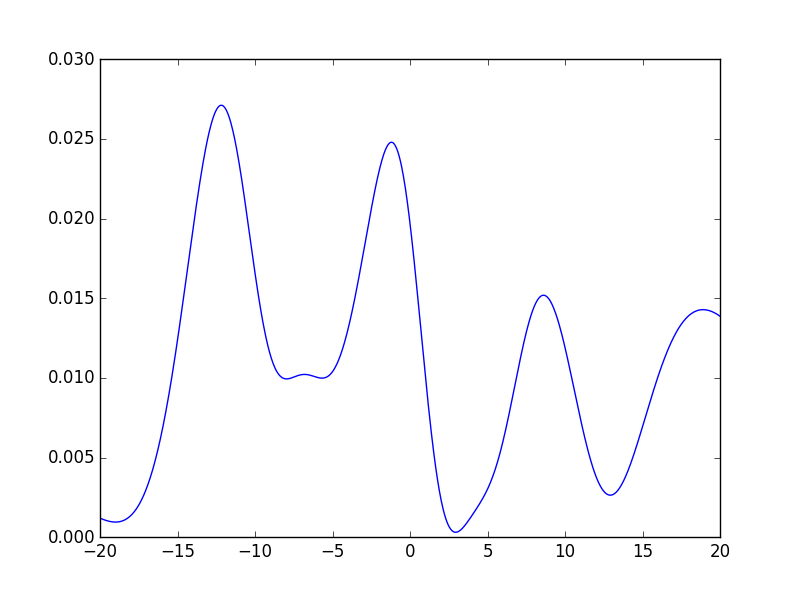
\includegraphics[scale=0.45]{figure_4.png}
    \caption{\label{fig:phase_2} Intensity profile of linear array of 4 antennae with 3 antennae in-phase and left-most antenna completely out of phase.}
\end{figure}

\subsubsection{Discussion}

These are the radiation patterns of interference between spherical waves produced with different phase between them. The result is a radiation pattern consisting of a strongly steered beam in one direction, plus a series of weaker beams, usually representing residual radiation in \textbf{unwanted} directions that can not participate in beam formation.
